\documentclass[a4paper]{article}
\usepackage{wasysym}
\usepackage[T1]{fontenc}
\usepackage[utf8]{inputenc}
\usepackage{lmodern}
\usepackage{graphicx}
\usepackage[english]{babel}
\usepackage{parskip}
\usepackage{hyperref}
\title{ShockSoc Lab Scripts\\ \huge{Rex's Fuzz Guitar Pedal}}
\author{Joel Fergusson}
\date{Rev 1.1}
\begin{document}
\maketitle

\newcommand{\ohm}{$\Omega$ }
\newcommand{\micro}{$\mu$ }

\section{Introduction}

	This lab aims to guide the reader through the construction of their 
	own distortion guitar pedal called Rex's Fuzz, based on a circuit by 
	Jack Orman\footnote{\url{http://www.muzique.com/schem/rex.gif}} of 
	the same name. ShockSoc will provide all the parts for 
	the construction of the provided circuit, but there's nothing 
	stopping the reader from extending or modifying the design to suit 
	their requirements. 
	
	The photo below is a photo of the prototype only. All the internals 
	are the same, but the components given to the participants will 
	include a stomp switch (which I didn't have available). Also, 
	the case will be different. 
	
	\begin{figure}[ht]
		\centering
		\includegraphics[width=0.8\textwidth]{DSCF7302.JPG}
		\caption{The prototype unit}
		\label{fig:schematic}
	\end{figure}
	
	The unit consists of two 6.35" Jack sockets -- one for the input one 
	for the output -- an LED that turns on when the unit is on, a foot 
	switch to toggle the unit, and two dials. These dials control the 
	drive (amount of distortion) and the level (volume of output).

\section{Circuit}
	Figure \ref{fig:schematic} shows the circuit diagram of the pedal.
	
	\begin{figure}[ht]
		\centering
		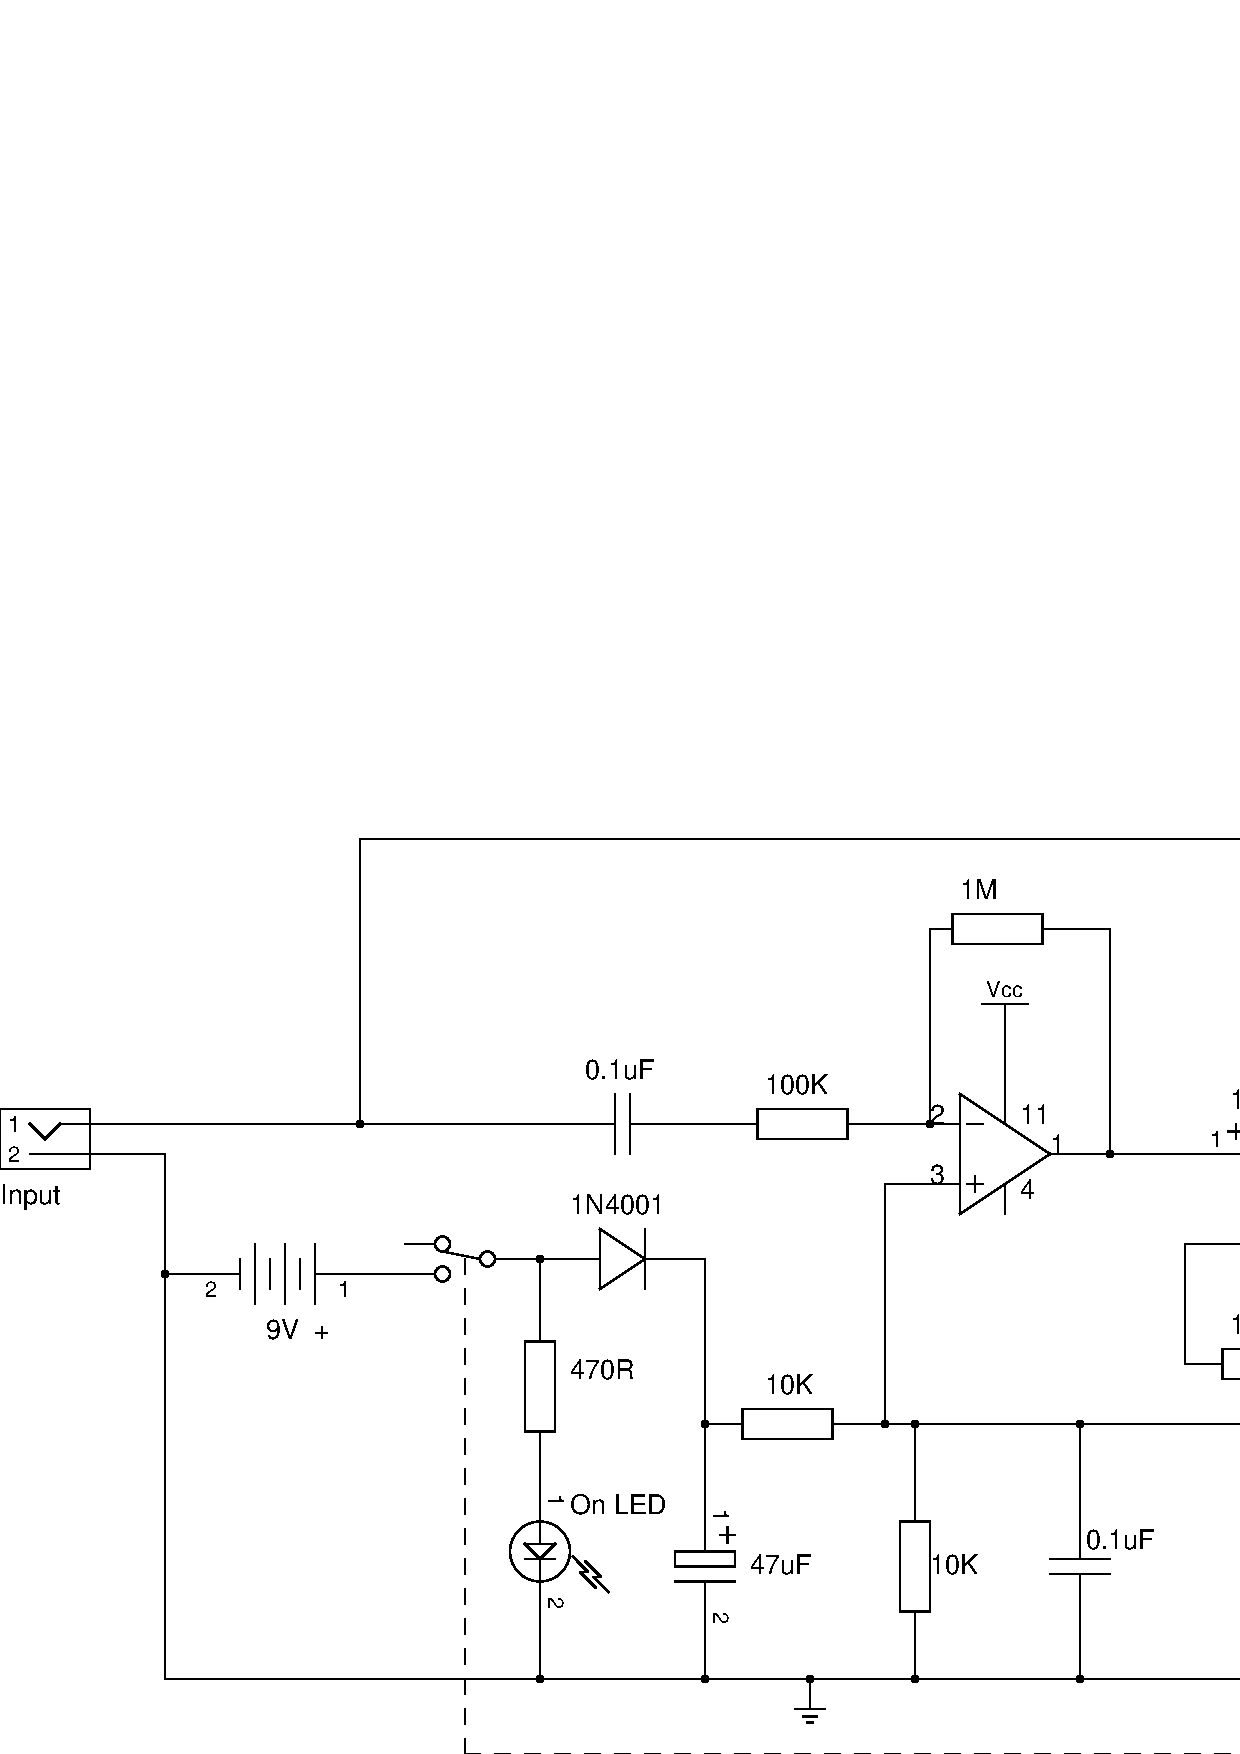
\includegraphics[angle=90, scale=0.18]{schematic.png}
		\caption{The circuit diagram}
		\label{fig:schematic}
	\end{figure}

	Some important notes of the diagram: 
	\begin{itemize}
		\item 	The ON LED and the associated 
				470\ohm resistor can be omitted if the reader doesn't want their 
				pedal to light up when in use. This will also save battery life.
	
		\item 	The op-amps can be from a dual circuit single-supply op-amp, hence
				the single power connections, one to V\_cc and one to ground.
				An LM358\footnote{\url{http://www.fairchildsemi.com/ds/LM/LM258.pdf}}
				chip is provided for the construction, but as this will be placed
				in an IC socket and not soldered directly, the reader may want to
				upgrade theirs to a higher spec chip. However, given the low bandwidths
				and gain require for this circuit, and the fact that it's a distortion pedal
				so noise is not entirely discouraged, it may not be worth the effort and 
				expense.
	\end{itemize}
	
	The operation of and theory behind the circuit left as an exercise for the reader,
	but feel free to ask if you don't understand it.
	\newpage
\section{Circuit construction}

	Provided with the components should be a piece of strip board measuring
	13 strips of 24 holes. This should exactly fit into the holding slots 
	inside the case provided. 
	
	This lab script does include a diagram for the stripboard layout, shown in figure
	\ref{fig:stripboard}. However, the reader is most welcome to ignore it and design
	their own. 
	
	\textbf{Please read the soldering guidelines below before soldering, they are 
	important and useful!}
	
	Figure \ref{fig:stripboard} shows the suggested stripboard layout, and Table 
	\ref{tab:values} shows the related component values. To explain the diagram,
	the red crosses are where the copper track on the board should be broken using 
	the strip cutters in the labs (they look like drill bits with handles). The 
	green lines are wires that connect two tracks together. Use solid-core wire for 
	those where possible. The orientation of each component is shown where it matters 
	(ICs, electrolytic capacitors, diodes, etc.). The black, blue or red arrows 
	leaving the board denote 
	wires to external components. These can be either solid- or multi-core wire. 
	
	\begin{figure}[ht]
		\centering
		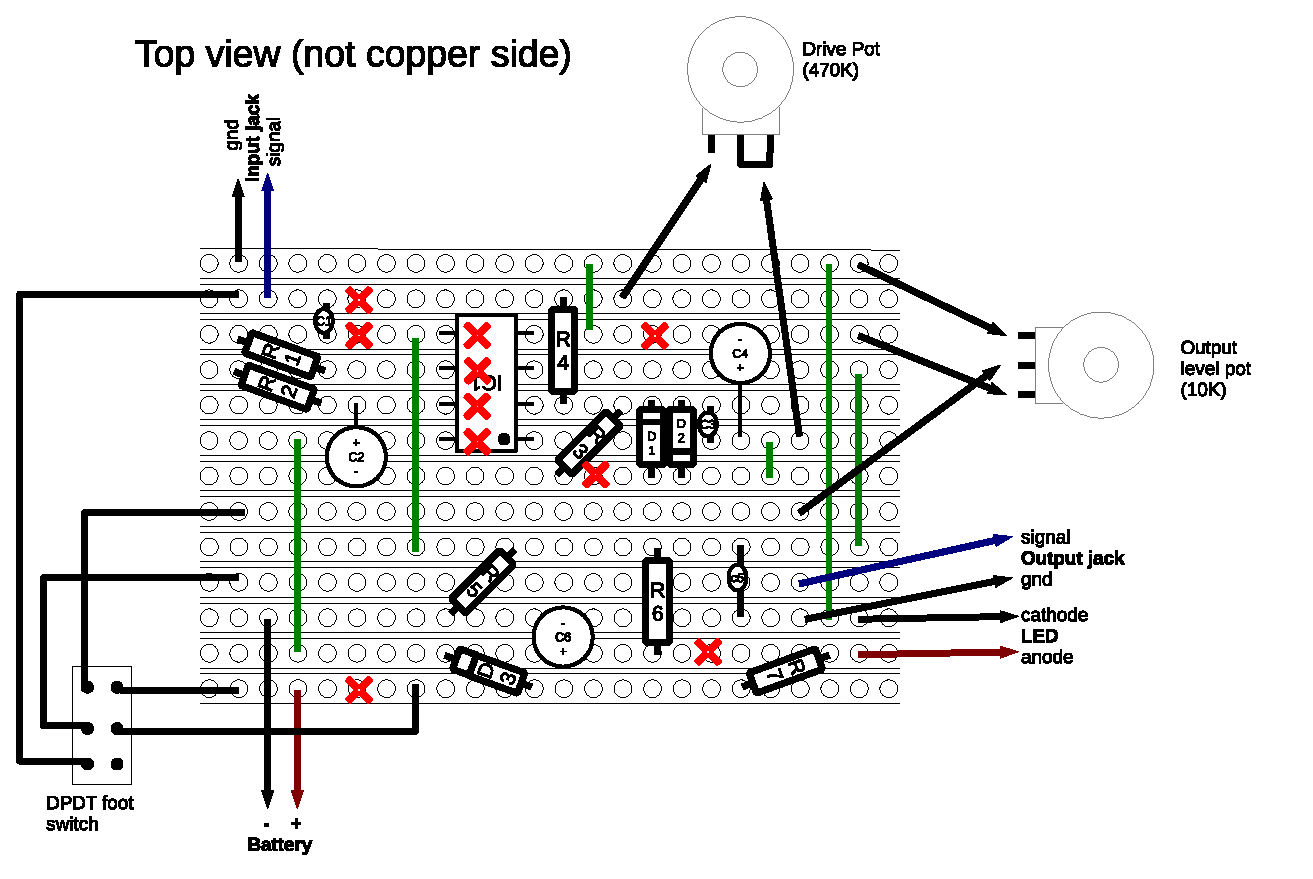
\includegraphics[angle=90, scale=0.9]{stripboard.eps}
		\caption{The suggested stripboard layout}
		\label{fig:stripboard}
	\end{figure}
	
	\begin{table}[h]
		\centering
		\begin{tabular}{ll}
			\textbf{Component Name} & \textbf{Value} 			\\ \hline
			R1             & 100K\ohm  	\\
			R2             & 1M\ohm    	\\
			R3, R4, R5, R6 & 10K\ohm   	\\
			R7             & 470\ohm  		\\
			C1, C5         & 0.1\micro F 	\\
			C2, C4         & 1\micro F   	\\
			C3             & 47pF  			\\
			C6             & 47\micro F  	\\
			D1, D2         & 1N914 			\\
			D3             & 1N4001     
		\end{tabular}
		\caption{The component values for the stripboard layout}
		\label{tab:values}
	\end{table}
	
	\subsection{Soldering Guidelines}
		Please read this carefully before soldering. They will make it 
		notably easier and less error prone. 
		
		\begin{itemize}
			\item 	Polarity: be careful about the polarity of all the relevant components.
					It's an easy mistake to make, but sometimes a difficult one to debug and fix.
					
			\item	The op-amp chip should not be soldered directly to the board. Instead, solder 
					the chip socket provided.
					
			\item	Try and keep the components flush to the board as you solder them. This will make 
					your circuit neater and less likely to have short circuits. 
			
			\item 	If there is a track break (red cross) on a hole next to a component, try
					to cut the track \textit{before} soldering in the component. 
					
			\item	Before soldering the wires that lead to the external components like the LED, 
					potentiometers or switch, remember to slip the heatshrink tubing on. If you're
					unfamiliar with heatshrink tubing, this video will show you how to use it: 
					\url{https://www.youtube.com/watch?v=ArtAEjgSDSU}
					
			\item 	If you're designing your own layout or have made a mistake and need to solder in
					different hole, try to avoid soldering the the edge holes on a row. This is because 
					when the circuit is placed in the case, the slots that hold the board in place will 
					infringe on this space. 
					
			\item	Make sure you've got enough length in the wires leading to the external components 
					to allow them to be mounted in the desired place in the case.
					
			\item If you don't understand anything, ask! 
		\end{itemize}
		
\section{Case construction}
	The case design is largely down to the reader. Listed here are the diameters of the holes needed
	for each component to be exposed:
	%TODO: Check these diameters are correct!
	\begin{table}[h]
		\centering
		\begin{tabular}{lc}
			\textbf{Component}  & \textbf{\diameter mm} \\ \hline
			Potentiometer  & 7              \\
			Switch         & 12.5           \\
			LED            & 5             \\
			Jack Socket    & 8            
		\end{tabular}
	\end{table}
\end{document}













